\section{Dataset}
\label{thedataset}

The dataset on which the analysis has been developed is an aggregated log of mobile phone
calls and short text messages with their geographical source and destination points.

The dataset is composed of several files, each one containing information of one specific day
within the observation period of two months (november and december 2013).

%% todo: inserire grid, nodes, edges

In each file, a row describes the connection strength between two geographical areas in the area surrounding Milan (Italy) during a time period of 10 minutes within the day.

The concept of connection strength between two areas is not formally defined: it is a decimal value proportional to the number of calls and sms sent from one area to another one.

Geographic areas are identified by a logical grid of $10.000$ squared areas 
% (with area $10.000m^2$) 
% todo: controllare numero
identified by an integer number $i \in [0, 9999]$ such that
$ i / 100 $ and $ i \% 100 $ are respectively the  
x and y coordinates of the node.

Therefore the format of each line is:

\begin{verbatim}
timestamp \t sourceNode	\t 	destNode \t strength
\end{verbatim}

where timestamp is the time in milliseconds describing the first millisecond of the period described.
To sum up, the dataset describes a number of directed weighted graphs over
the nodes of the geopgraphical grid, one for each 10-minutes long interval
in the 2 months observation period. The total size of the dataset is around 345GB.
\newpage

\section{Data distributions analysis}
\label{ds_analysis}

In order to understand the possibility of finding such communities, 
we run some analysis on the weights of the arcs.
This analysis has been done over weights of arcs, 
neglecting temporarely their probabilisitc nature but considering
them just as common random variables.
We consider this analysis as executed on a stochastic process with discrete times and discrete values in [0,1].

In Fig. \ref{fig:analysis} some statistics on the process are shown. Please notice that the analysis has been done over 
a certain day of the dataset (to be precise, the 15th of november), thus is not comprehensive and is only meant to give 
an indication of the shape of the data.
\begin{figure}[H]
\centering
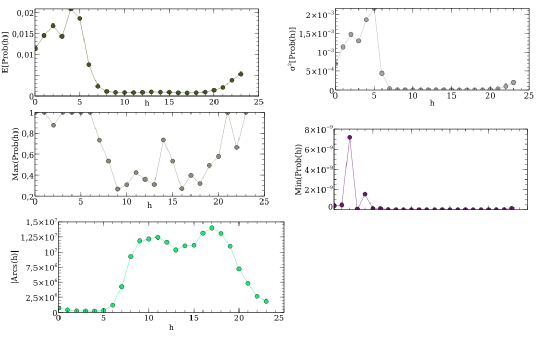
\includegraphics[scale=0.7]{arcsanalysis.png}
\caption{\label{fig:analysis}Plots on the probabilities detected in the graph. Subfigures are numberd from (a) to (e) going from left to right and from top to bottom.}
\end{figure}

In (a) we show the empirical mean for every hour of the day taken into consideration. It is possible to notice that, during
night hours, the average probability experiences a spike, probably indicating that the number of outgoing arcs in these 
hours is lower than usual. This hypothesis is confirmed by the plot in (e), in which the total number of non-null arcs
for a graph over an hour is shown.
Part (b), instead, shows the behaviour of the variance on the probability of the arcs in different hours. While during
working hours the variance is very low (with several outgoing arcs converging towards the average), it grows
in non-working hours.
In (c) and in (d) we show, instead, the maximum and minimum probability values of the arcs for any hour graphs. Particularly interesting
is (c), in which it is possible to notice that, in the hours with high traffic, some spikes in traffic exist, while
the minima always remain in the order of $10^-9$ 
